\documentclass{article}

\usepackage{graphicx}
\usepackage[hypcap]{caption}
\usepackage{listings}
\usepackage{float}
\floatstyle{plaintop}
\restylefloat{table}
\usepackage{caption,subcaption}
\usepackage[margin=1.6in]{geometry}

\title{Experimental Design and Data Analysis: Assignment 5}
\author{Andrew Bedard(2566978) \& Simone van Gompel(2567525) \\ Group 19}

\begin{document}

  \maketitle

  \section*{Exercise 1}
    \subsection*{1}
    Using the data obtained from nauseatable.txt, we create a data frame consisting of two columns and 304 rows. One column contains an indicator, 0 for negative, 1 for positive, that a patient suffered from nausea, and the other column indicates the medicine the patient received.
    
    \subsection*{2}
    By using the R command xtabs(\textasciitilde medicine+nausea) we are able to create a contingency table of our data so far. As we can see in figure 1
    \begin{figure}[H]
    \begin{lstlisting}[language=R]
                     No Nausea Nausea
Chlorpromazine             100     52
Pentobarbital(100mg)        32     35
Pentobarbital(150mg)        48     37
    \end{lstlisting}
    \caption{Contingency table for all 3 drugs, and their effect}
    \label{fig:cont_table}
    \end{figure}
    
    On this contingency table we are able to perform Pearson's Chi-squared test, performing this test we obtain a p-value of 0.0364, suggesting we reject the null hypothesis that there is no significant difference in the effect of the drugs.
    
    \subsection*{3}
    We may also now perform a permutation test in order to determine whether the different medications work equally well against nausea. This is done by permuting the medicine labels, and once again using the Chi-squared test as our test statistic. We obtain the following histogram of values for the Chi-squared test, after permuting labels, and repeated 1000 times:
    
    \begin{figure}[H]
          \centering
          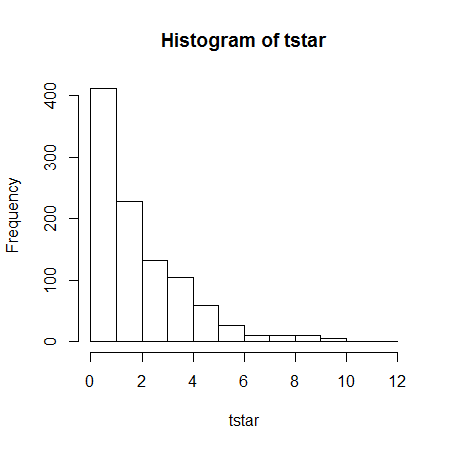
\includegraphics[scale=0.6]{../results/1_3.png}
          \caption{Histogram of Chi-squared values of permuted labels}
          \label{fig:Htgrm}
      \end{figure} 
    
By summing up all values obtained from this test which are greater than the value obtained by simply performing the Chi-squared test on the original data which is 6.62, then dividing by the number of samples performed, we create a p-value simulated in a boot-strap fashion. The resulting p-value is 0.033, which suggests that we reject the null hypothesis that all medicines work equally well.
    
    \subsection*{4}
    \begin{itemize}
    \item the p-value obtained from the Chi-square test for contingency tables was 0.0364
    \item the p-value obtained from the permutation test was 0.033
    \end{itemize}
    As a permutation test is a bootstrap type test, and the distribution of the test statistic is approximated by simulation we do see a variation in the p-values for each method, however for large replications for our permutation test on our data, this difference should not be significant enough to change our results. This is due to the fact that all our values of figure: 1 are greater than 1, and more than 80\% of our values are greater than 5, which allows us to approximate the test statistic by the Chi-squared test.
  \section*{Exercise 2}
    \subsection*{1}
    After reading in the data contained in airpollution.txt, we examine the relationship between all variables in figure \ref{fig:pairs}
      \begin{figure}[H]
          \centering
          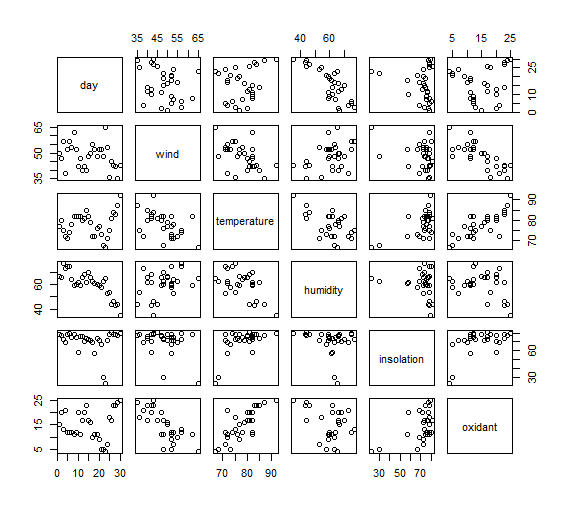
\includegraphics[scale=0.6]{../results/2_1.png}
          \caption{Pairplot of the airpollution data}
          \label{fig:pairs}
      \end{figure} 
      
   As seen in above figure \ref{fig:pairs} there are many variables that have a visible linear relationship with oxidant, like temperature for example, this gives a strong indication that a linear model may be appropriate for this data.
   
    \subsection*{2}
   With the response variable in this data being Oxidant, for each of the explanatory variables \textbf{day, wind, temperature, humidity, insulation}, we create a simple linear regression model, and using the method outline in R-Code section: \ref{sec:RE2} we stepwise extend the model by adding an additional explanatory variable based on increasing the determination coefficient of our model. 
    
        \begin{table}[H]
    \begin{center}
    \begin{tabular}{|ll|}
        \hline
        Variable & $R^2$ \\
        \hline 
        Step1&\\
        \hline
        Oxidant\textasciitilde day & 0.0109 \\
        Oxidant\textasciitilde wind & 0.5863 \\
        Oxidant\textasciitilde temperature & 0.5760 \\
        Oxidant\textasciitilde humidity & 0.1240 \\
        Oxidant\textasciitilde insulation & 0.2551 \\
        \hline
        Step2&\\
        \hline 
        Oxidant\textasciitilde wind+day & 0.5988 \\
        Oxidant\textasciitilde wind+temperature & 0.7773 \\
        Oxidant\textasciitilde wind+humidity & 0.5913 \\
        Oxidant\textasciitilde wind+insulation & 0.6613 \\
        \hline
        Step3&\\
        \hline 
        Oxidant\textasciitilde wind+temperature+day & 0.7958 \\
        Oxidant\textasciitilde wind+temperature+humidity & 0.7963 \\
        Oxidant\textasciitilde wind+temperature+insulation & 0.7816 \\
        \hline
        Step4&\\
        \hline
        Oxidant\textasciitilde wind+temperature+humidity+day &  0.7974\\
        Oxidant\textasciitilde wind+temperature+humidity+insulation & 0.7979\\
        \hline
    \end{tabular}
    \caption{Step-up method}
    \label{table:step-up2}
    \end{center}
    \end{table}
    
    As can be seen by Table: \ref{table:step-up2} after each step we add another variable to the model when that variable increases our determination coefficient $R^2$, however the gains in the determination coefficient $R^2$ do not increase in any significant way after step 3, so this is where we stop. From this model we then obtain the estimates for our model parameters from a summary of our linear model:
	\begin{figure}[H]
	\begin{lstlisting}[language=R]
Coefficients:
             Estimate Std. Error t value Pr(>|t|)    
(Intercept) -16.60697   13.07154  -1.270    0.215    
wind         -0.44620    0.08513  -5.241 1.78e-05 ***
temperature   0.60190    0.11764   5.117 2.47e-05 ***
humidity      0.09850    0.06316   1.559    0.131    
---
Signif. codes:  
0 ‘***’ 0.001 ‘**’ 0.01 ‘*’ 0.05 ‘.’ 0.1 ‘ ’ 1
    \end{lstlisting}
    \caption{Summary of computed linear model}
    \label{table:twotwo}
    \end{figure}
    
    Our model is thus:
    $$Oxidant = -16.6069 -0.4462*wind + 0.6019*temperature + 0.0985*humidity + error$$

    Using a similar method to the previous section, we now stepwise decrease a model that includes all explanatory variables, and using a test of the form $H_0: \beta_i = 0$ we select variables to exclude from the model until we reject the null hypothesis for all explanatory variables still contained in the model.
    
    	\begin{figure}[H]
    	\begin{subfigure}[b]{1\linewidth}
	\begin{lstlisting}[language=R]
Coefficients:
             Estimate Std. Error t value Pr(>|t|)    
(Intercept) -12.04010   21.20961  -0.568  0.57553    
day          -0.02997    0.13995  -0.214  0.83227    
wind         -0.44749    0.09103  -4.916 5.14e-05 ***
temperature   0.55714    0.15347   3.630  0.00133 ** 
humidity      0.06818    0.13336   0.511  0.61384    
insolation    0.01822    0.05583   0.326  0.74694    
---

    \end{lstlisting}
    \caption{Day has the highest p-value, we eliminate it from the model}
    \end{subfigure}
    
        	\begin{subfigure}[b]{1\linewidth}
	\begin{lstlisting}[language=R]
             Estimate Std. Error t value Pr(>|t|)    
(Intercept) -15.49370   13.50647  -1.147  0.26219    
wind         -0.44291    0.08678  -5.104 2.85e-05 ***
temperature   0.56933    0.13977   4.073  0.00041 ***
humidity      0.09292    0.06535   1.422  0.16743    
insolation    0.02275    0.05067   0.449  0.65728    
---

    \end{lstlisting}
    \caption{Insulation has the highest p-value, we eliminate it from the model}
    \end{subfigure}
    \caption{Steps 1 and 2 of step-down method}
    \end{figure}
    \begin{figure}[H]
           \begin{subfigure}[b]{1\linewidth}
	\begin{lstlisting}[language=R]
             Estimate Std. Error t value Pr(>|t|)    
(Intercept) -16.60697   13.07154  -1.270    0.215    
wind         -0.44620    0.08513  -5.241 1.78e-05 ***
temperature   0.60190    0.11764   5.117 2.47e-05 ***
humidity      0.09850    0.06316   1.559    0.131    
---
    \end{lstlisting}
    \caption{Humidity has the highest p-value, we eliminate it from the model}
   \end{subfigure}

 	\begin{subfigure}[b]{1\linewidth}
	\begin{lstlisting}[language=R]
            Estimate Std. Error t value Pr(>|t|)    
(Intercept) -5.20334   11.11810  -0.468    0.644    
wind        -0.42706    0.08645  -4.940 3.58e-05 ***
temperature  0.52035    0.10813   4.812 5.05e-05 ***
---
Signif. codes:  
0 ‘***’ 0.001 ‘**’ 0.01 ‘*’ 0.05 ‘.’ 0.1 ‘ ’ 1
    \end{lstlisting}
    \caption{Summary of computed full linear model minus day, insulation and humidity, and all remaining variables have a p-value less than 0.05}
    \end{subfigure}
    \caption{Steps 3 and 4 of step-down method}
    \label{fig:stepdown2}
    \end{figure}
 
 Thus as illustrated in figure 5 and 6, at each step we remove a single explanatory variable that has a p-value greater than 0.05, or rather, a variable for which we fail to reject the null hypothesis that $\beta_i = 0$.
 
 By this method we obtain the model:
 $$Oxidant = -5.2033 -0.4271*wind+0.5204*temperature+error$$
 
    \subsection*{4}
    The models that we obtained through the step up and step down methods are as follows
    \begin{itemize}
    \item For the step up model we obtained:
    $$Oxidant = -16.6069 -0.4462*wind + 0.6019*temperature + 0.0985*humidity+error$$
    \item For the step down model we obtained:
    $$Oxidant = -5.2033 -0.4271*wind+0.5204*temperature+error$$
    \end{itemize}
    
    The model that we would choose would be the one obtained through the step up method: $Oxidant = -16.6069 -0.4462*wind + 0.6019*temperature + 0.0985*humidity+error$. This is mainly due to the fact that our $R^2$ value indicates that the model does improve with the addition of humidity, as seen in part 2, even though we failed to reject the null hypothesis for this factor being 0 in the step-down method, thus our determination coefficient is 0.7963 as opposed to the step-down model which gives a determination coefficient of 0.7773.
    
    \subsection*{5}
    
    We investigate the qqplot and the fitted plot of the residuals from the model we chose and obtained the following:
    
          \begin{figure}[H]
          \centering
          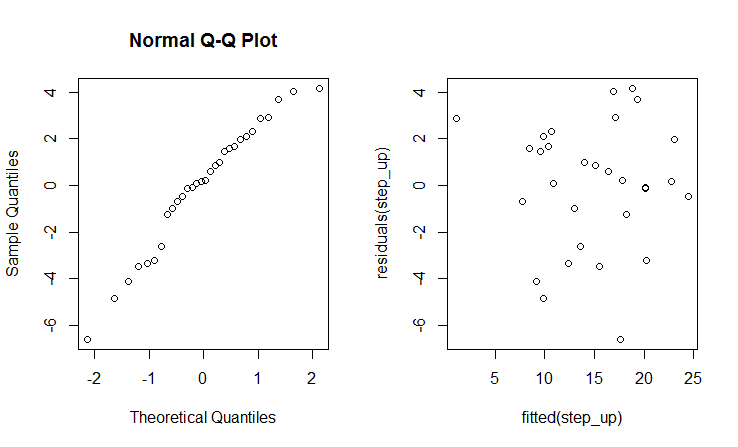
\includegraphics[scale=0.6]{../results/2_5.png}
                    \label{fig:qqresid}
          \caption{QQ and fitted plots of residuals}

      \end{figure} 
    
As seen in figure 7, both our Normall qq plot and fitted plot suggest that our residuals are normal, which would suggest that our linear model is in fact appropriate.

  \section*{Exercise 3}
    \subsection*{1}
    The data from genal2.txt was read in and transformed into a data frame with two columns as outlined in the R-Code section \ref{sec:RE3}
    \subsection*{2}
    Making a box plot of the data frame created form the previous section we obtain the following:
    	\begin{figure}[H]
    		\centering
    		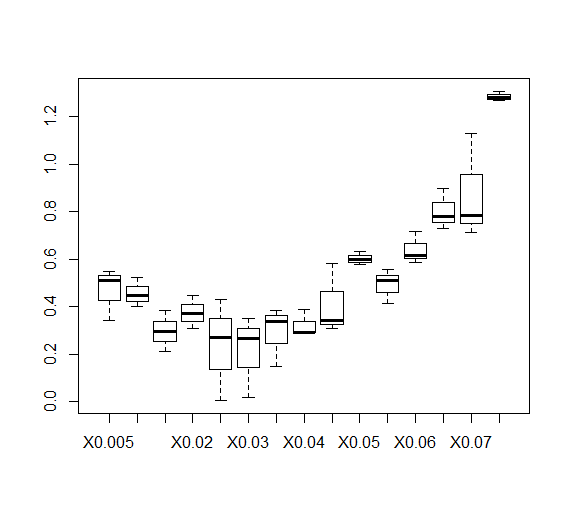
\includegraphics[scale=0.4]{../results/3_2.png}
    		\label{BoxMut}
    		\caption{Boxplot of 15 mutation probabilities}
   
    	\end{figure}
    Clearly from the curved shape of the box plot figure:8, we can see that the dependence of y on \textit{mut} is obviously not linear, but appears with a distinct curve.
    \subsection*{3}
    Next we fit a multiple linear regression model for y on $mut$ and $mut^2$ using the code outlined in R-Code Section \ref{sec:RE3}. We obtain the following table:
    \begin{figure}[H]
    \begin{lstlisting}[language=R]
Coefficients:
             Estimate Std. Error t value Pr(>|t|)    
(Intercept)   0.60538    0.06317   9.583 3.94e-12 ***
mut         -23.78772    3.63372  -6.546 6.50e-08 ***
mut2        417.96154   44.16824   9.463 5.68e-12 ***
---
Signif. codes:  
0 ‘***’ 0.001 ‘**’ 0.01 ‘*’ 0.05 ‘.’ 0.1 ‘ ’ 1    
    \end{lstlisting}
    \caption{Summary of multiple linear model for y on mut and $mut^2$}
    \end{figure}
    
    Which from the estimates we can conclude our model is should be:
    $$Y = 0.60538 - 23.78772*mut + 417.96154*mut^2 + error$$
    \subsection*{4}
    
    We now make a plot of our model as a function of the mutation probability seen in figure \ref{PlotMut}.
        \begin{figure}[H]
    	\centering
    	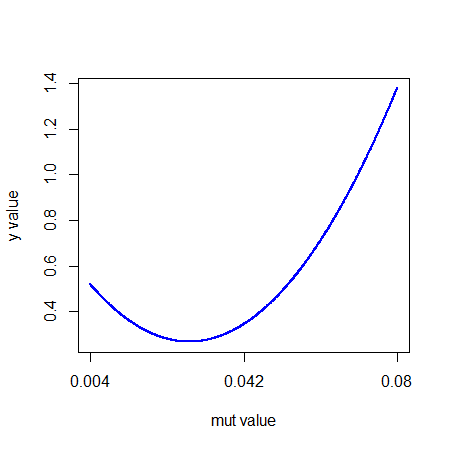
\includegraphics[scale=0.6]{../results/3_4.png}
    	\caption{Plot of multiple linear regression model for values of mut between 0.004 and 0.08}
    	\label{PlotMut}
    	\end{figure}    
    
    By taking the value of mut at which the y value given is lowest, we obtain the optimal mutation probability, which we have calculated to be 0.0284
    \subsection*{5}
    \begin{itemize}
    \item parameters were estimated from our data, being $\beta_0=0.60538, \beta_1=-23.78772, \beta_2=417.96154$
    \item Had we estimated the parameters from the data with the mutation probabilities defined as labels rather than numerical values we would have at estimated at least 16 parameters. This is because, as we saw in figure 8 the relationship between y and $mut$ is clearly not linear, but looks quadratic in nature, thus we would need \textbf{at least} 1 of our 15 $mut$ variables to be quadratic. To obtain the most accurate model, we would likely have estimated 30 parameters, that is, a $mut_i$ and $mut_i^2$ for each label $i$.
    \end{itemize}

  \section*{Exercise 4}
    The dataset \textit{expensescrime} is exolored.
    The response variable is \textit{expend} and the rest are independent variables.
    In Fig\ref{fig:PairsCrime} the pairs plot of the data is shown.
    
        \begin{figure}[H]
        \centering
        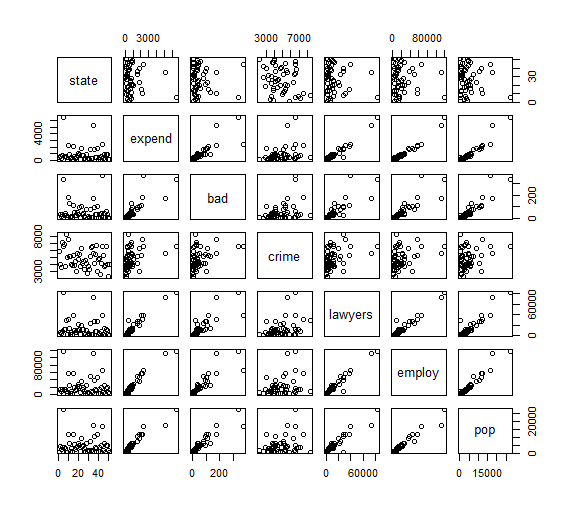
\includegraphics[scale=0.6]{../results/4_pairs.png}
        \caption{The pairs plot}
        \label{fig:PairsCrime}
    \end{figure}
    
    From figure \ref{fig:PairsCrime} we can see that many variables have a linear relationship with our response variable, suggesting that it would be appropriate to use a linear model. This figure also shows that many variables are co-linear. Indeed if we inspect pop and employ they have a very strictly linear relationship, and further from figure 12 we can see that their correlation is almost perfect at 0.97, which complicates our process and would suggest that we should not use both variables in our model. 
 
      	\begin{figure}[H]
	\begin{lstlisting}[language=R]
         bad crime lawyers employ  pop expend
bad     1.00  0.37    0.83   0.87 0.92   0.83
crime   0.37  1.00    0.38   0.31 0.28   0.33
lawyers 0.83  0.38    1.00   0.97 0.93   0.97
employ  0.87  0.31    0.97   1.00 0.97   0.98
pop     0.92  0.28    0.93   0.97 1.00   0.95
expend  0.83  0.33    0.97   0.98 0.95   1.00    
       \end{lstlisting}
    \caption{Correlation table}
    \label{table:cortble}
    \end{figure} 
    
    To create the linear regression model, we will utilize both the step-up and step-down methods to ensure that our model is as optimal as we can make it.
    The following is the result of the step-up method, similar as is illustrated in exercise 2
    \begin{table}[H]
    \begin{center}
    \begin{tabular}{|ll|}
        \hline
        Variable & $R^2$ \\
        \hline 
        Step1&\\
        \hline
        Expend\textasciitilde Pop & 0.9073 \\
        Expend\textasciitilde Employ & 0.954 \\
        Expend\textasciitilde Lawyers & 0.9373 \\
        Expend\textasciitilde Crime & 0.1119 \\
        Expend\textasciitilde Bad & 0.6964 \\
        \hline
        Step2&\\
        \hline 
        Expend\textasciitilde Employ+Pop & 0.9543 \\
        Expend\textasciitilde Employ+Lawyers & 0.9632 \\
        Expend\textasciitilde Employ+Crime & 0.9551 \\
        Expend\textasciitilde Employ+Bad & 0.9551 \\
        \hline
        Step3&\\
        \hline 
        Expend\textasciitilde Employ+Lawyers+Pop & 0.9637 \\
        Expend\textasciitilde Employ+Lawyers+Crime & 0.9632 \\
        Expend\textasciitilde Employ+Lawyers+Bad & 0.9639 \\
        \hline
    \end{tabular}
    \caption{Step-up method}
    \label{table:step-up}
    \end{center}
    \end{table}
    
    Clearly from table 2 we can conclude that we do not achieve significant gains in our determination coefficient after adding employ and lawyers to our model, so we once again obtain our parameters from the following table:
    
\begin{figure}[H]
	\begin{lstlisting}[language=R]
Coefficients:
              Estimate Std. Error t value Pr(>|t|)    
(Intercept) -1.107e+02  4.257e+01  -2.600  0.01236 *  
employ       2.971e-02  5.114e-03   5.810 4.89e-07 ***
lawyers      2.686e-02  7.757e-03   3.463  0.00113 ** 
---
Signif. codes:  
0 ‘***’ 0.001 ‘**’ 0.01 ‘*’ 0.05 ‘.’ 0.1 ‘ ’ 1
    \end{lstlisting}
    \caption{Summary of computed linear model}
    \label{table:fourstepup}
    \end{figure}
    
Thus as a result of this step-up method, our model is:

$$Expend = -1.107e^2 + 2.971e^{-2}*employ + 2.686e^{-2}*lawyers + error$$    
    
    Again as illustrated in exercise 2, again we perform the step down method, eliminating variables that fail to reject the null hypothesis that their parameters are equal to 0.
    
    
    \begin{table}[H]
    \begin{center}
    \begin{tabular}{|ll|}
        \hline
        Variable & \textit{p} \\
        \hline 
        Step1&\\
        \hline
        Expend\textasciitilde Employ+Lawyers+Bad+Pop+Crime & $R^2 = 0.9675$ \\
        Employ & 0.00354 \\
        Lawyers & 0.00592 \\
        Bad & 0.02719 \\
        Pop & 0.03184 \\
        Crime & 0.25534\\
        \hline
        Step2&\\
        \hline 
        Expend\textasciitilde Employ+Lawyers+Bad+Pop & $R^2 = 0.9666$ \\
        Employ & 0.00380 \\
        Lawyers & 0.00106 \\
        Bad & 0.05402 \\
        Pop & 0.06012 \\
        \hline
        Step3&\\
        \hline 
        Expend\textasciitilde Employ+Lawyers+Bad & $R^2 = 0.9639$ \\
        Employ & 1.2e-06 \\
        Lawyers & 0.00147 \\
        Bad & 0.34496 \\
        \hline
        Step4&\\
        \hline 
        Expend\textasciitilde Employ+Lawyers+Bad & $R^2 = 0.9632$ \\
        Employ & 4.89e-07 \\
        Lawyers & 0.00113 \\
        \hline
    \end{tabular}
    \caption{Step-down method}
    \label{table:step-down}
    \end{center}
    \end{table}
    Both methods end up with the same formula, namely Expend\textasciitilde Employ+Lawyer.
    The results of the formula for Expend is as follows:
    \[
      Expend = -1.107e^2 + 2.971e^{-2} * Employ + 2.686e^{-2} * Lawyers + error
    \]
    \\

	Now that we have created a model, we should test if this result is reasonable, we have already concluded that some variables have collinearity, and we may still investigate whether there are influence points or outliers that may cause issues for us. Consider the following scatter plot of all variables left in our model:
	
	    \begin{figure}[H]
        \centering
        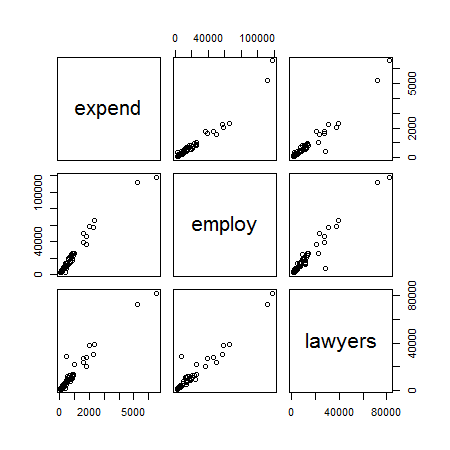
\includegraphics[scale=0.5]{../results/4_99.png}
        \caption{Scatter plots of all variables}
        \label{fig:4collin}
    \end{figure}
    
    It is very clear from figure \ref{fig:4collin} lawyers and employ may be collinear, and this is what we find in actuality, they are correlated by a factor of 0.9657, which is likely too high for them to both be in our model. So referring back to Table 2, we will conclude that our model shall only include employ, thus from the following table :
  	\begin{figure}[H]
	\begin{lstlisting}[language=R]
  
    Coefficients:
              Estimate Std. Error t value Pr(>|t|)    
(Intercept) -1.167e+02  4.706e+01   -2.48   0.0166 *  
employ       4.681e-02  1.469e-03   31.87   <2e-16 ***
---
Signif. codes:  
0 ‘***’ 0.001 ‘**’ 0.01 ‘*’ 0.05 ‘.’ 0.1 ‘ ’ 1
    \end{lstlisting}
    \caption{Summary of computed linear model}
    \label{table:fournew}
    \end{figure}
    
	we conclude that our model should now be:
	
	$$Expend = -1.167e^{2} - 4.681e^{-2}*employ + error$$
	
	which yields only a slightly lower value for $R^2$ which is 0.954.
    
    The influence points can be found by cook's distance, seen in Fig\ref{fig:4cook}.
    There is only significant data point that can influence the methods used.
    \begin{figure}[H]
        \centering
        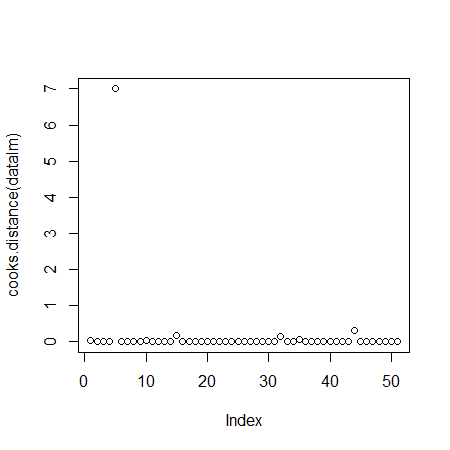
\includegraphics[scale=0.4]{../results/4_cook.png}
        \caption{The cook's distance}
        \label{fig:4cook}
    \end{figure}

    The residuals can be found in Fig\ref{fig:4res}, which indicate that the data is not linearly correlated. None of the data in the plots is randomly scattered, This is backed up by Fig\ref{fig:4qq}
    \begin{figure}[H]
        \centering
        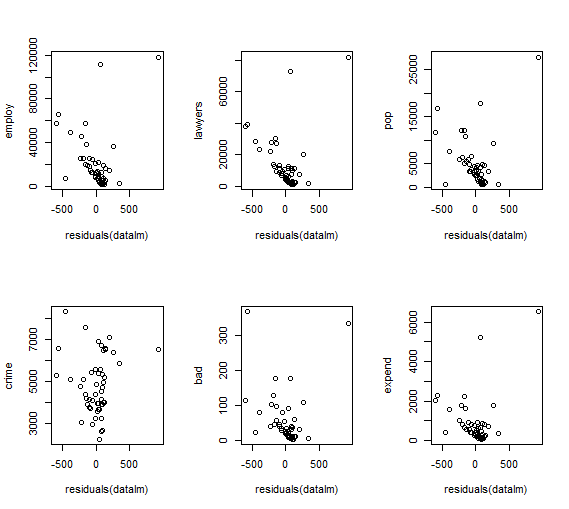
\includegraphics[scale=0.6]{../results/4_res.png}
        \caption{The residuals of the regression}
        \label{fig:4res}
    \end{figure}
    
    \begin{figure}[H]
        \centering
        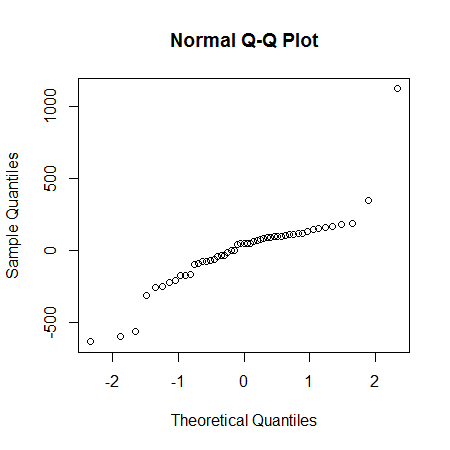
\includegraphics[scale=0.4]{../results/4_qq.png}
        \caption{QQ-plot of the residuals}
        \label{fig:4qq}
    \end{figure}
    
    Thus we conclude that our model is reasonable.
    
  \section{R-Code}
    \subsection{Exercise 1}\label{sec:RE1}
      \begin{lstlisting}[language=R]
      data = read.table("nauseatable.txt")

#1.1

rnames = rownames(data)
nausea = c()
medicin = c()
for (j in 1:length(data[,1])){
  for (i in 1:length(data[1,])){
    nausea = c(nausea, rep(i-1, data[j,i]))
    medicin = c(medicin, rep(rnames[j], data[j,i]))
  }
}
medicin <- factor(medicin)
nausea.frame=data.frame(nausea,medicin)

#1.2

#Create contingency table
cont_table = xtabs(~medicin+nausea)

#Contingency table has to be in matrix form for calculations
cont_matrix = matrix(c(100,52,32,35,48,37), byrow=TRUE, ncol=2 ,nrow=3, 
                     dimnames=list(c(rownames(data)[1],
                                     rownames(data)[2],rownames(data)[3]),c("No Nausea","Nausea")))


#chisquared test for contigency matrix
chisq.test(cont_matrix)

#1.3

teststat.obs = chisq.test(xtabs(~medicin+nausea))[[1]]

B = 1000
tstar=numeric(B)
for (i in 1:B)
{
  medstar = sample(medicin) ## permuting labels
  tstar[i] = chisq.test(xtabs(~nausea+medstar))[[1]]
}


hist(tstar)

#p-value

sum(tstar>teststat.obs)/B

#1.4

#chisquared test for contigency matrix with simulated p value
chisq.test(cont_matrix,simulate.p.value=TRUE)
      \end{lstlisting}
    \subsection{Exercise 2}\label{sec:RE2}
      \begin{lstlisting}[language=R]
      data = read.table("airpollution.txt")

#2.1
pairs(data)

#2.2

#create simple models, plot for reference
par(mfrow=c(2,3))

oxday = lm(oxidant~day, data=data)
plot(oxidant~day, data=data); abline(oxday)

oxwind = lm(oxidant~wind, data=data)
plot(oxidant~wind, data=data); abline(oxwind)

oxtemp = lm(oxidant~temperature, data=data)
plot(oxidant~temperature, data=data); abline(oxtemp)

oxhum = lm(oxidant~humidity, data=data)
plot(oxidant~humidity, data=data); abline(oxhum)

oxins = lm(oxidant~insolation, data=data)
plot(oxidant~insolation, data=data); abline(oxins)

summary(oxday)$r.squared
summary(oxwind)$r.squared
summary(oxtemp)$r.squared
summary(oxhum)$r.squared
summary(oxins)$r.squared

#wind has highest R squared, so add to model

summary(lm(oxidant~wind+day,data=data))$r.squared
summary(lm(oxidant~wind+temperature,data=data))$r.squared
summary(lm(oxidant~wind+humidity,data=data))$r.squared
summary(lm(oxidant~wind+insolation,data=data))$r.squared

#temperature has highest R squared, add to model

summary(lm(oxidant~wind+temperature+day ,data=data))$r.squared
summary(lm(oxidant~wind+temperature+humidity ,data=data))$r.squared
summary(lm(oxidant~wind+temperature+insolation ,data=data))$r.squared

#adding humidity still increased R squared, add to model

summary(lm(oxidant~wind+temperature+humidity+day ,data=data))$r.squared
summary(lm(oxidant~wind+temperature+humidity+insolation ,data=data))$r.squared

#adding either day or insolation yields insignificant explanatory variables
#so we stop at previous step

summary(lm(oxidant~wind+temperature+humidity,data=data))

#summary gives coefficients of model in estimate column

#2.3

summary(lm(oxidant~day+wind+temperature+humidity+insolation, data=data))

#Try removing day, (highest p-value)
summary(lm(oxidant~wind+temperature+humidity+insolation, data=data))

#removing insolation, (highest p-value)
summary(lm(oxidant~wind+temperature+humidity, data=data))

#removing humidity, p-value too high still
summary(lm(oxidant~wind+temperature, data=data))

#2.4
#Present stepwise increase, less variables, but similar result

#2.5
step_up = lm(oxidant~wind+temperature+humidity,data=data)

par(mfrow=c(1,2))
qqnorm(residuals(step_up))
plot(fitted(step_up),residuals(step_up))
      \end{lstlisting}
    \subsection{Exercise 3}\label{sec:RE3}
      \begin{lstlisting}[language=R]
      data = read.table("genal2.txt")

#3.1
y = c()
mut = c()
# gives X0.005, so not useable
names = names(data)
length(data[1,])
length(data[,1])
for (i in 1:length(data[1,])){
  for (j in 1:length(data[,1])){
    y = c(y, data[j,i])
    mut = c(mut, 0.005*i)
  }
}
genal2frame=data.frame(y,mut)

#3.2
boxplot(data)

#3.3
genal2frame$mut2=genal2frame$mut^2
genal2lm=lm(y~mut+mut2,data=genal2frame)
summary(genal2lm)


#3.4

func1 = function(x) (0.605358-23.78772*x+417.96154*x^2)

B=1000
ypoints = numeric(B)
xpoints = seq(0.004,0.08,length=B)

for (i in 1:B){
  ypoints[i] = func1(xpoints[i])
}


plot(ypoints, xaxt = "n",xlab="mut value",ylab="y value",pch=20, cex=0.2, col="blue")
axis(1,at=c(1,500,1000), labels=c(xpoints[1],round(xpoints[500],digits = 4),xpoints[1000]))
#Optimal mutation value correspons to xpoint where y is smallest
round(xpoints[match(min(ypoints),ypoints)],digits=4)
      \end{lstlisting}
    \subsection{Exercise 4}\label{sec:RE4}
      \begin{lstlisting}[language=R]
      library('corrplot')
data = read.table("expensescrime.txt", header=T)
attach(data)

# looking at correlations, 
# the correlation plot is on the last line of the program
pairs(data)
dataframe = data.frame(bad,crime,lawyers,employ,pop,expend)
round(cor(dataframe), 2)

# step-up algorithm
# examine r squared
summary(lm(expend~pop))$r.squared
summary(lm(expend~employ))$r.squared
summary(lm(expend~lawyers))$r.squared
summary(lm(expend~crime))$r.squared
summary(lm(expend~bad))$r.squared

summary(lm(expend~employ+pop))$r.squared
summary(lm(expend~employ+lawyers))$r.squared
summary(lm(expend~employ+crime))$r.squared
summary(lm(expend~employ+bad))$r.squared

summary(lm(expend~employ+lawyers+pop))$r.squared
summary(lm(expend~employ+lawyers+crime))$r.squared
summary(lm(expend~employ+lawyers+bad))$r.squared

summary(lm(expend~employ+lawyers))

# step-down algorithm
# same result as step-up so continue with this
summary(lm(expend~employ+lawyers+bad+pop+crime))
summary(lm(expend~employ+lawyers+bad+pop))
summary(lm(expend~employ+lawyers+bad))
summary(lm(expend~employ+lawyers))

# influence points are the ones that stand out in cooks distance
datalm = lm(expend~employ)
round(cooks.distance(datalm),2)
par(mfrow=c(1,1))
plot(cooks.distance(datalm))

# problems with colinearty, the corrplot is on the bottom
round(cor(data[,3:7]),2)

# looking at the different residuals
par(mfrow=c(1,1))
plot(residuals(datalm),employ)
par(mfrow=c(2,2))
plot(residuals(datalm),lawyers)
plot(residuals(datalm),pop)
plot(residuals(datalm),crime)
plot(residuals(datalm),bad)
par(mfrow=c(1,2))
plot(residuals(datalm),expend)
plot(residuals(datalm),fitted(datalm))
par(mfrow=c(1,1))
qqnorm(residuals(datalm))

pairs(~expend+employ+lawyers)
cor(employ,lawyers)
      \end{lstlisting}
\end{document}
